\chapter{Administration Module}
\minitoc
\clearpage
\section{Introduction}
This chapter presents the Administration module, which gives administrators full control over user governance and project-manager assignments. The module is organized around two main pages: Dashboard and Projects.

\section{Sprint Backlog}
The administration backlog focused on governance and control features:
\begin{center}
	\renewcommand{\arraystretch}{1.2}
	\begin{tabular}{|l|>{\raggedright\arraybackslash}p{9.5cm}|l|}
		\hline
		\textbf{ID} & \textbf{Backlog Item} & \textbf{Priority} \\
		\hline
		AB-01 & Build a dashboard to monitor account distribution by role (Admin, HR, Project Manager). & High \\
		\hline
		AB-02 & Allow administrators to create, edit, and delete user accounts. & High \\
		\hline
		AB-03 & Provide controlled user editing while preventing direct password modification from the listing workflow. & Medium \\
		\hline
		AB-04 & Allow administrators to assign project managers to projects. & High \\
		\hline
		AB-05 & Add filtering, pagination, and scalable table behavior for large datasets. & Medium \\
		\hline
	\end{tabular}
\end{center}

\section{Sprint Design}
The module design separates account governance and project assignment into dedicated interfaces for clarity and operational efficiency.
To communicate the React implementation clearly, this section presents interface mockups created with Excalidraw.

\subsection{Dashboard module design}
The Dashboard page was designed as the administration control center. It contains user summary cards (Admin, HR, and Project Manager counts) and a users table with account-management actions.

\begin{figure}[H]
	\centering
	\IfFileExists{assets/admin/dashboard-module-design-mockup.jpg}{%
		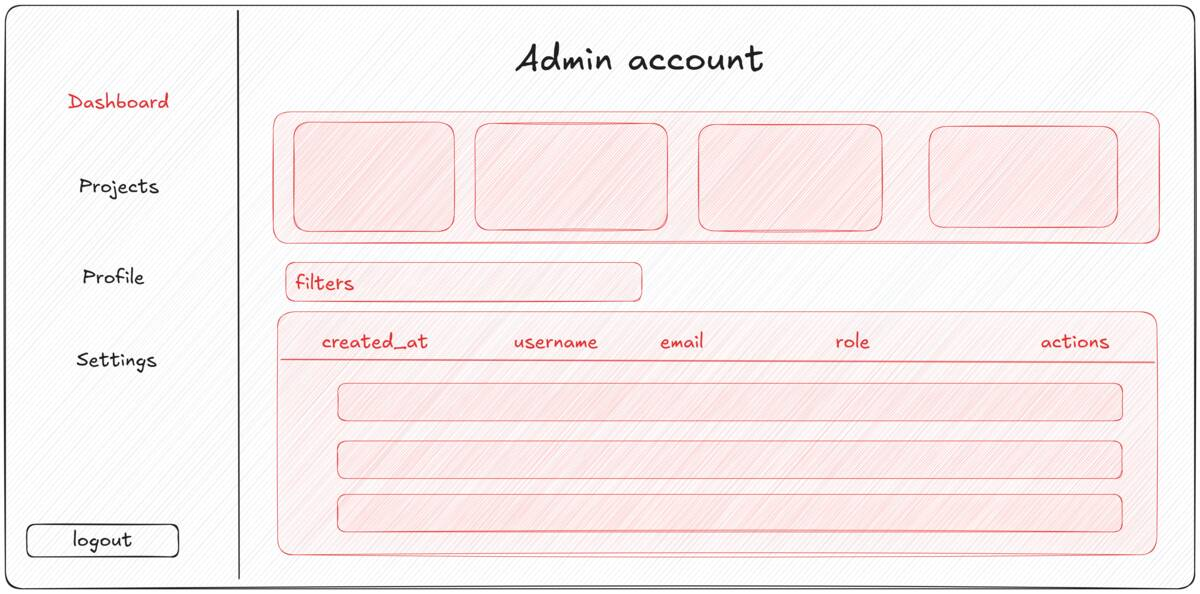
\includegraphics[width=0.92\textwidth,height=0.46\textheight,keepaspectratio]{assets/admin/dashboard-module-design-mockup.jpg}
	}{%
		\fbox{\parbox{0.9\textwidth}{
				\centering
				\vspace{1.6cm}
				\textit{Missing file: assets/admin/dashboard-module-design-mockup.jpg}\\
				\textit{Insert Dashboard module design mockup (Excalidraw).}
				\vspace{1.6cm}
		}}
	}
	\caption{Dashboard Module Design Mockup}
	\label{fig:admin-dashboard-design-mockup}
\end{figure}

\subsection{Projects module design}
The Projects page was designed to manage project ownership by project managers. It contains a projects table where each row provides an action that opens a dedicated assignment page.

\begin{figure}[H]
	\centering
	\IfFileExists{assets/admin/projects-module-design-mockup.jpg}{%
		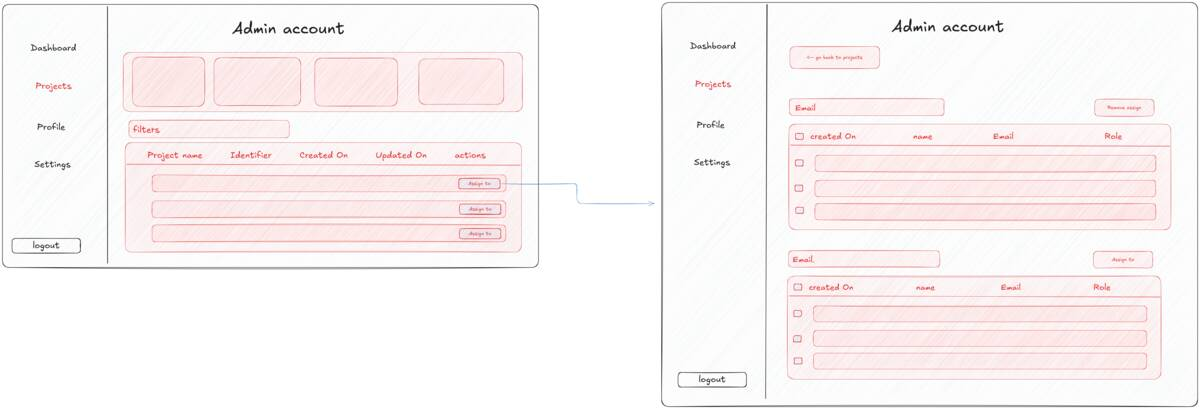
\includegraphics[width=0.92\textwidth,height=0.46\textheight,keepaspectratio]{assets/admin/projects-module-design-mockup.jpg}
	}{%
		\fbox{\parbox{0.9\textwidth}{
				\centering
				\vspace{1.6cm}
				\textit{Missing file: assets/admin/projects-module-design-mockup.jpg}\\
				\textit{Insert Projects module design mockup (Excalidraw).}
				\vspace{1.6cm}
		}}
	}
	\caption{Projects Module Design Mockup}
	\label{fig:admin-projects-design-mockup}
\end{figure}

\section{Conception}
\subsection{Administration use case diagram}
The administration use case model defines the main administrator interactions: create, edit, and delete accounts; view role distribution; consult projects; and assign project managers.

\begin{figure}[H]
	\centering
	\IfFileExists{diagrams/ch5-admin-use-case.jpg}{%
		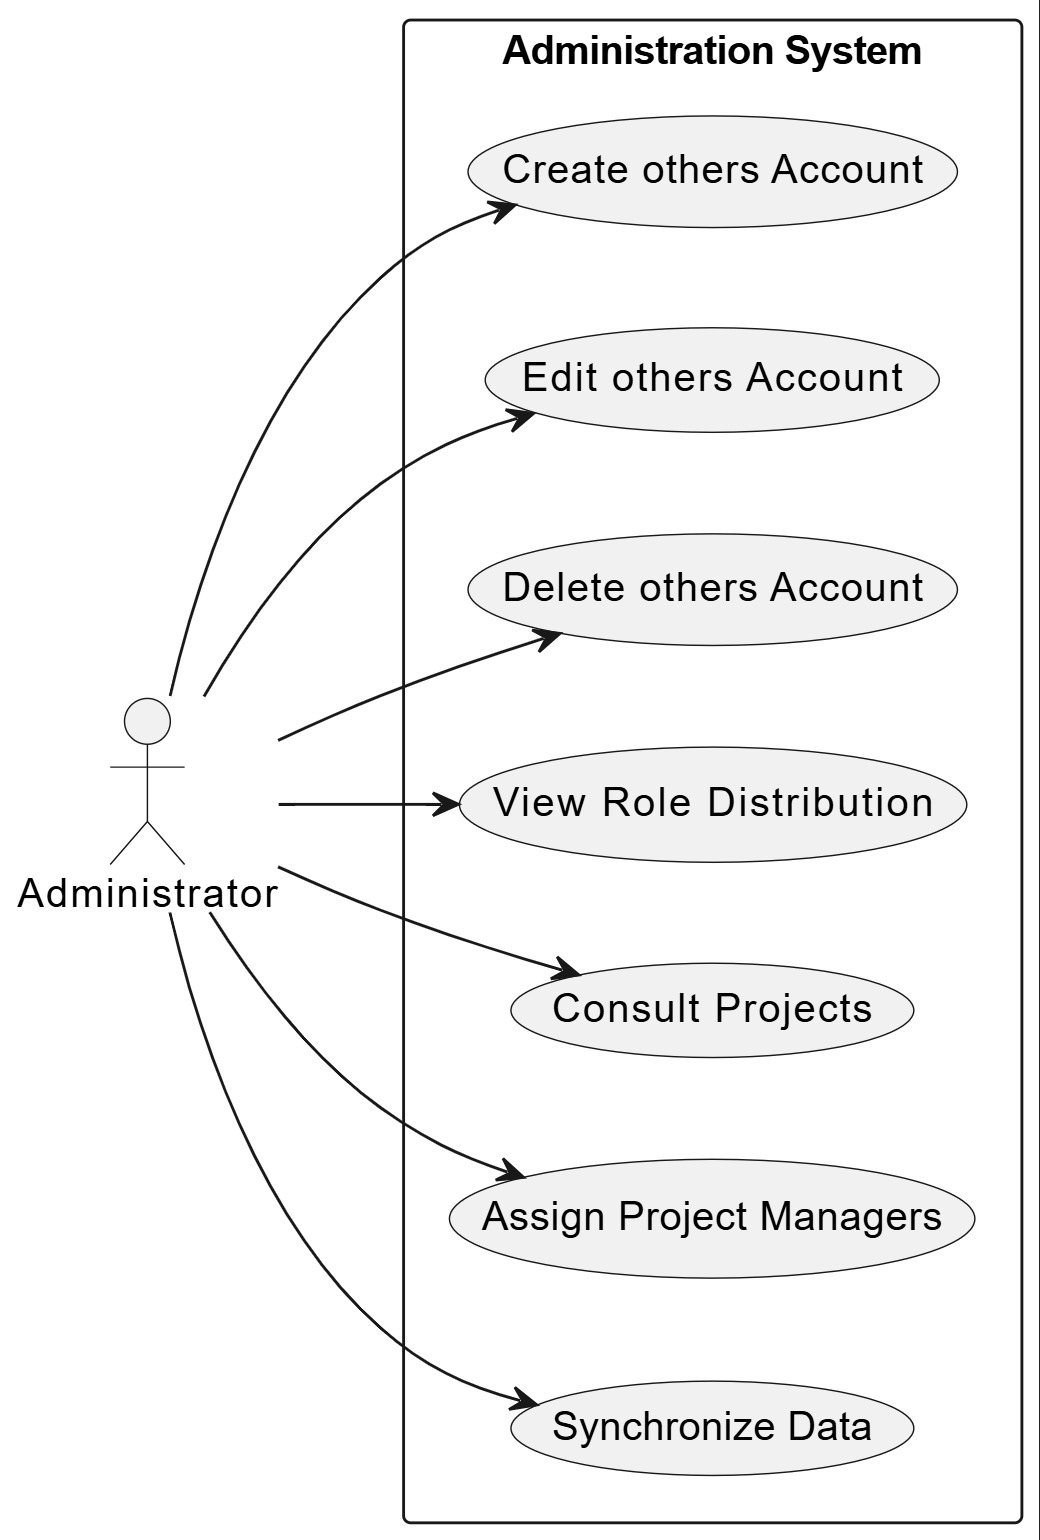
\includegraphics[width=0.92\textwidth,height=0.52\textheight,keepaspectratio]{diagrams/ch5-admin-use-case.jpg}
	}{%
		\fbox{\parbox{0.9\textwidth}{
				\centering
				\vspace{1.6cm}
				\textit{Missing file: diagrams/ch5-admin-use-case.jpg}\\
				\textit{Insert Administration module use case diagram.}
				\vspace{1.6cm}
		}}
	}
	\caption{Administration Module Use Case Diagram}
	\label{fig:admin-use-case}
\end{figure}
Figure~\ref{fig:admin-use-case} summarizes administrator actions and governance scope.

\section{Sprint Realization}
\subsection{Implementation outcomes}
\begin{itemize}[noitemsep]
	\item Implemented Dashboard module with role-based user summary cards.
	\item Implemented Users table with create, edit, and delete account actions.
	\item Implemented edit flow for user information without password update through table actions.
	\item Implemented Projects table and project-manager assignment page.
	\item Implemented Settings page actions to synchronize and update unified database data from BioTime and EasyProject.
	\item Integrated filters, pagination, and TanStack Query caching across tables.
\end{itemize}

\subsection{Administration dashboard and users interface}
\begin{figure}[H]
	\centering
	\IfFileExists{assets/admin/dashboard-users.jpg}{%
		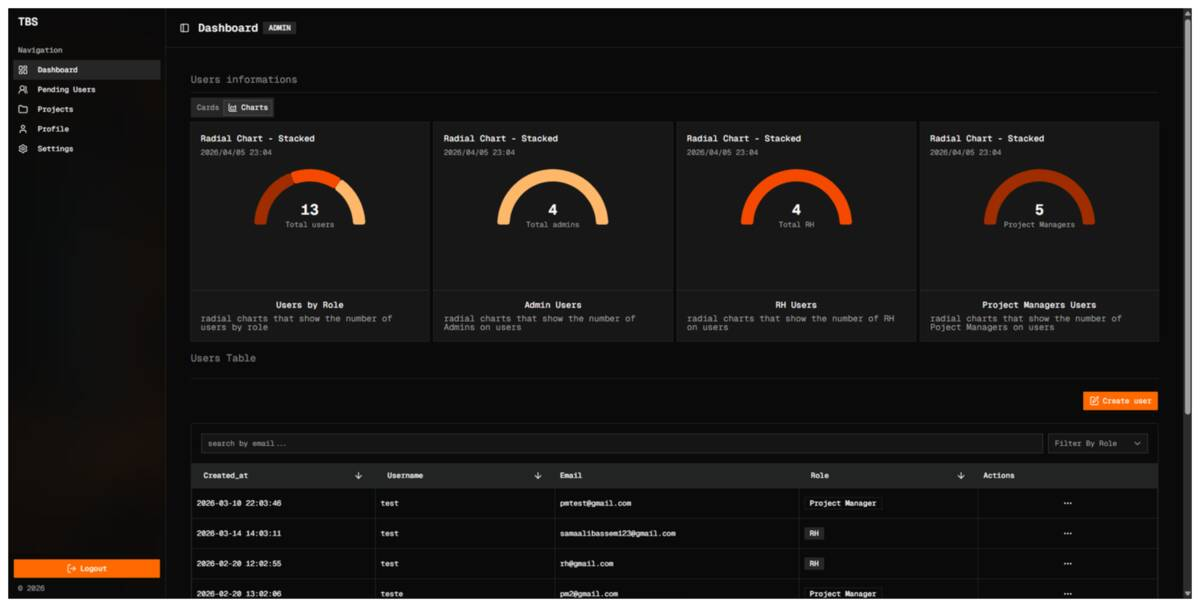
\includegraphics[width=0.92\textwidth,height=0.50\textheight,keepaspectratio]{assets/admin/dashboard-users.jpg}
	}{%
		\fbox{\parbox{0.9\textwidth}{
				\centering
				\vspace{1.6cm}
				\textit{Missing file: assets/admin/dashboard-users.jpg}\\
				\textit{Insert dashboard screenshot with user cards and users table.}
				\vspace{1.6cm}
		}}
	}
	\caption{Administration Dashboard: User Cards and Users Table}
	\label{fig:admin-dashboard-users}
\end{figure}
Figure~\ref{fig:admin-dashboard-users} shows role-distribution cards and the user-management table with edit/delete actions.

\subsection{Projects interface}
\begin{figure}[H]
	\centering
	\IfFileExists{assets/admin/projects-page.jpg}{%
		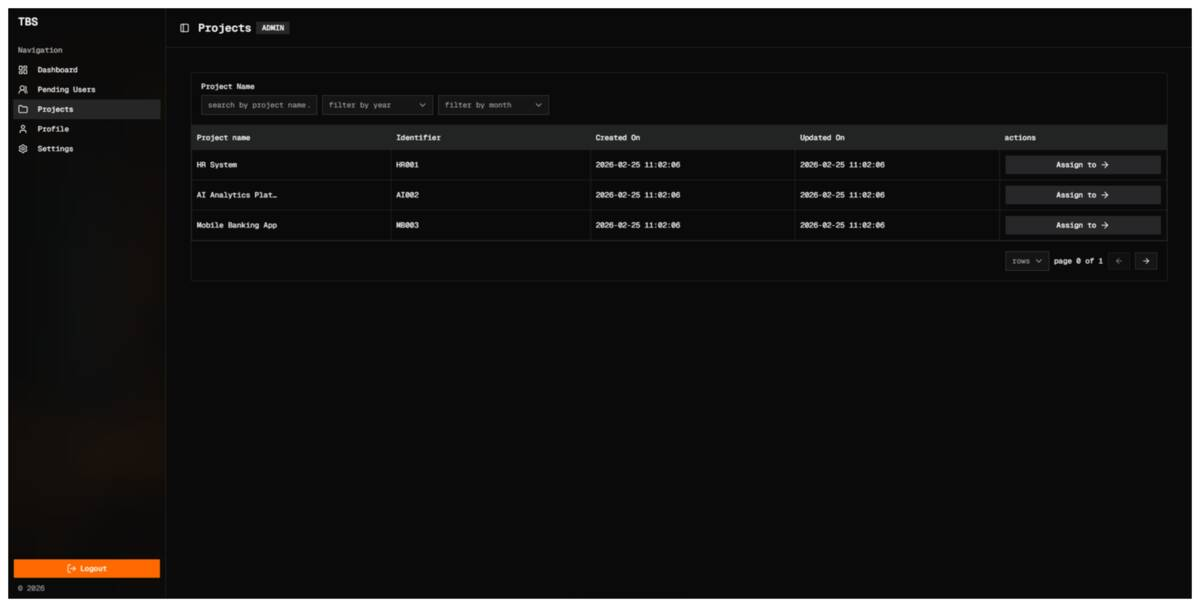
\includegraphics[width=0.92\textwidth,height=0.50\textheight,keepaspectratio]{assets/admin/projects-page.jpg}
	}{%
		\fbox{\parbox{0.9\textwidth}{
				\centering
				\vspace{1.6cm}
				\textit{Missing file: assets/admin/projects-page.jpg}\\
				\textit{Insert Administration Projects page screenshot.}
				\vspace{1.6cm}
		}}
	}
	\caption{Administration Projects Page}
	\label{fig:admin-projects-page}
\end{figure}
Figure~\ref{fig:admin-projects-page} presents the projects table used to select projects for assignment actions.

\subsection{Assign project interface}
\begin{figure}[H]
	\centering
	\IfFileExists{assets/admin/assign-project-page.jpg}{%
		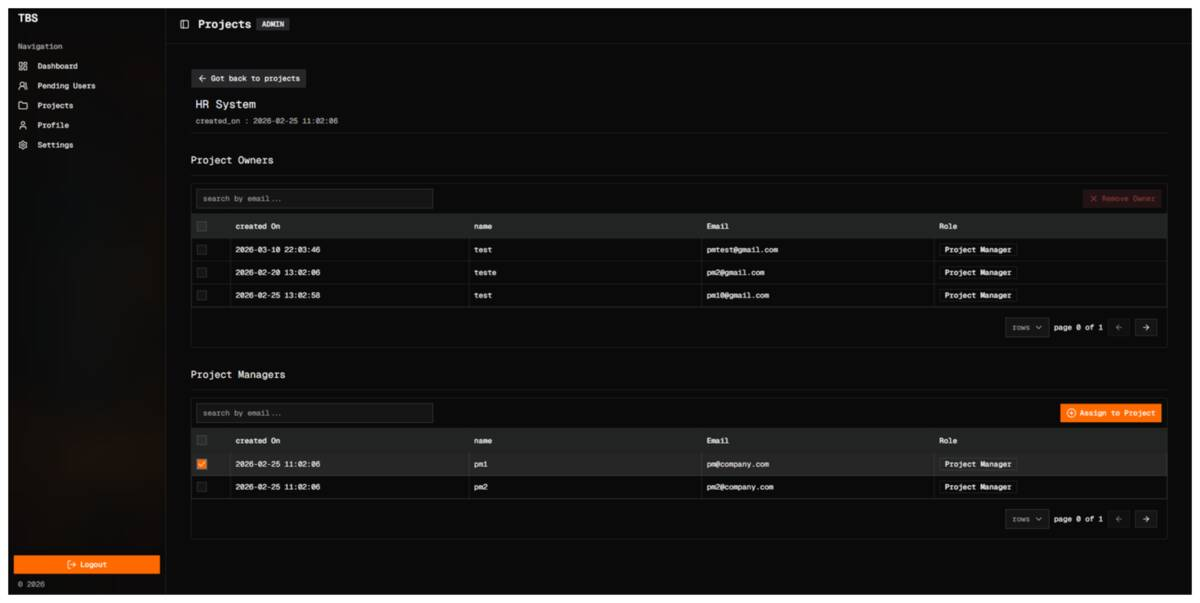
\includegraphics[width=0.92\textwidth,height=0.50\textheight,keepaspectratio]{assets/admin/assign-project-page.jpg}
	}{%
		\fbox{\parbox{0.9\textwidth}{
				\centering
				\vspace{1.6cm}
				\textit{Missing file: assets/admin/assign-project-page.jpg}\\
				\textit{Insert Assign Project page screenshot with project manager selection.}
				\vspace{1.6cm}
		}}
	}
	\caption{Assign Project Page}
	\label{fig:admin-assign-project-page}
\end{figure}
Figure~\ref{fig:admin-assign-project-page} illustrates assigning one or more project managers to the selected project.

\subsection{Settings page interface}
\begin{figure}[H]
	\centering
	\IfFileExists{assets/admin/settings-page.jpg}{%
		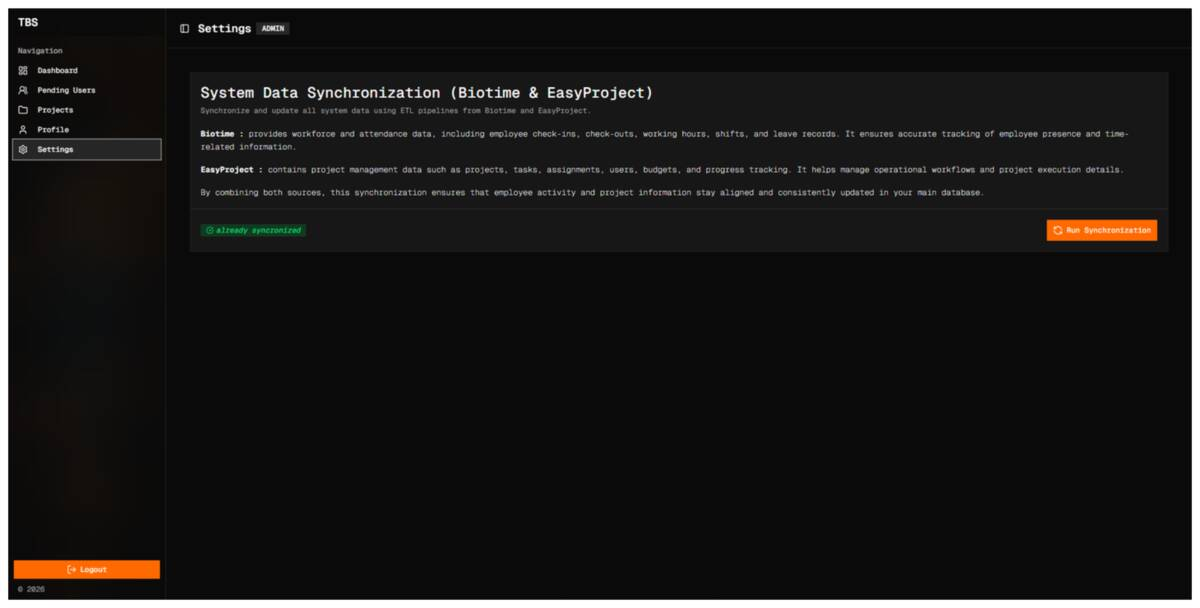
\includegraphics[width=0.92\textwidth,height=0.50\textheight,keepaspectratio]{assets/admin/settings-page.jpg}
	}{%
		\fbox{\parbox{0.9\textwidth}{
				\centering
				\vspace{1.6cm}
				\textit{Missing file: assets/admin/settings-page.jpg}\\
				\textit{Insert Settings page screenshot with BioTime and EasyProject synchronization/update actions.}
				\vspace{1.6cm}
		}}
	}
	\caption{Administration Settings Page for Data Synchronization}
	\label{fig:admin-settings-page}
\end{figure}
Figure~\ref{fig:admin-settings-page} presents the Settings interface where the administrator can trigger synchronization or update operations to refresh the unified database from BioTime and EasyProject.

\subsection{Filtering and  pagination interface}
\begin{figure}[H]
	\centering
	\IfFileExists{assets/admin/table-filters-pagination.jpg}{%
		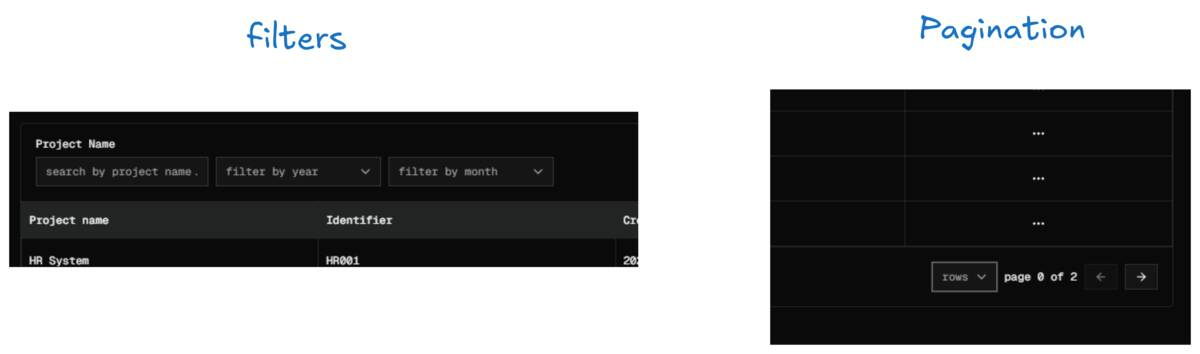
\includegraphics[width=0.92\textwidth,height=0.46\textheight,keepaspectratio]{assets/admin/table-filters-pagination.jpg}
	}{%
		\fbox{\parbox{0.9\textwidth}{
				\centering
				\vspace{1.6cm}
				\textit{Missing file: assets/admin/table-filters-pagination.jpg}\\
				\textit{Insert table filtering, pagination, and caching behavior illustration.}
				\vspace{1.6cm}
		}}
	}
	\caption{Filtering and Pagination}
	\label{fig:admin-table-performance}
\end{figure}
Figure~\ref{fig:admin-table-performance} summarizes large-dataset handling through filters, pagination, and TanStack Query caching.

\section{Conclusion}
The Administration module delivered complete governance capabilities for users and project assignments. With scalable tables, controlled actions, and cached data access, the module supports efficient administration even with large datasets.
